\documentclass[conference]{IEEEtran}
\usepackage{booktabs}
\usepackage{graphicx}
\usepackage{hyperref}
\hypersetup{hidelinks}
\usepackage{xcolor}
\usepackage{amsmath}
\usepackage{amssymb}
\usepackage{placeins}

% IEEE's narrow columns and full-width research tables can produce benign
% underfull-box diagnostics during float balancing.
\hbadness=10000
\vbadness=10000

\graphicspath{{../figures/}{figures/}}

\makeatletter
\long\def\@makecaption#1#2{%
  \footnotesize\centering
  \def\@tempa{table}%
  \ifx\@captype\@tempa
    Table~\thetable. #2\par
  \else
    Figure~\thefigure. #2\par
  \fi}
\makeatother

\title{EviCode: Understanding Verification Evidence for Machine-Generated Code}

\author{}

\begin{document}
\maketitle

\begin{abstract}
Generated programs must be checked before they can be trusted, yet the usual checks often depend on resources that are unavailable: similarity metrics need a trusted target-language reference, execution needs tests and runtimes, and formal verification needs specifications. This study asks what can still be learned directly from a source program and generated candidate. We use EviCode, a transparent analysis instrument, to compare observations of syntax, structure, control flow, operators, identifier roles, data flow, library calls, complexity, and tested behavior. Across 2,952 HumanEval-X verification pairs, reference-free static observations rank a correct translation above an incorrect one about 80\% of the time (ROC-AUC $=0.801$), but do not prove correctness. Once behavioral observations become available, accept/reject quality reaches 90.4\% F1. Collectively, the experiments reveal an empirical semantic information ladder: surface observations remove little uncertainty, language-normalized program properties provide inexpensive triage and diagnosis, and execution produces the largest reduction because it observes tested outcomes. The contribution is therefore an account of what each observation can establish, which uncertainty it reduces, and when acquiring it is worth the cost.
\end{abstract}

\begin{IEEEkeywords}
Generated-code verification, program translation, semantic evidence, uncertainty reduction, calibration, explainable software analytics.
\end{IEEEkeywords}

\section{Introduction}
Imagine a developer asks a large language model (LLM) to translate a Python function into Java. The candidate looks plausible, but no trusted Java translation exists, tests have not yet been written, and no Java expert is available to inspect it. Should the candidate be accepted, repaired, or rejected? Surface resemblance cannot answer: a translation can retain names and tree shape while changing one operator, or look different while preserving the intended behavior. Generation has produced code, but not the evidence needed to trust it.

Existing verification routes each require an unavailable resource. Similarity metrics normally compare a candidate with a trusted target-language reference, but such a reference may be exactly what generation is meant to create. Execution observes behavior but requires tests, runnable dependencies, and an appropriate environment. Formal verification can provide stronger guarantees, but requires specifications and analysis effort that are rarely available for routine generated candidates. This leaves an important pre-execution question: what semantic evidence can be obtained directly from the source program and candidate when no reference translation exists?

EviCode studies that question through \emph{reference-free verification}. It transforms each program into comparable evidence about validity, organization, control, computation, value roles, and value propagation, then treats confidence estimation as an analysis instrument. The scientific goal is not another classifier. It is to understand how partial observations accumulate, which semantic uncertainty each removes, and what each observation costs.

This problem has a close analogue in machine translation: \emph{quality estimation} (QE) predicts the quality of a generated translation from the source sentence and translation hypothesis when no reference translation is available~\cite{fonseca2019wmtqe,kepler2019openkiwi,ranasinghe2020transquest,rei2022cometkiwi}. EviCode adopts the same resource-aware question for neural code intelligence: can a generated target-language program be assessed directly from the source program and candidate, without a trusted target implementation at inference? The analogy clarifies both scope and novelty. EviCode does not introduce reference-free estimation itself; it extends that framing to programs, where correctness depends on syntax, control, computation, and behavior. It therefore exposes language-normalized observation families and studies how their information, cost, calibration, and complementarity accumulate, rather than treating quality estimation only as prediction of one end score.

This goal suggests a proposition rather than a conclusion: observations closer to program behavior should usually remove more uncertainty, but should also cost more to acquire. Conceptually, the study therefore tests the progression
\[
\begin{gathered}
\text{lexical form}\rightarrow\text{syntax}\rightarrow\text{program structure}\\[-0.2em]
\rightarrow\text{behavioral proxies}\rightarrow\text{execution}.
\end{gathered}
\]
The progression is not assumed to be monotonic or universal. The experiments measure whether it is recovered, where adjacent observations overlap, and how cost and availability constrain acquisition. Figure~\ref{fig:empirical-semantic-ladder} later reports the hierarchy that actually emerges.

The investigation develops three connected pieces of the resulting explanation:
\begin{itemize}
\item \textbf{Evidence-aggregation formulation.} A reference-free formulation of translated-code verification in which a source program and translated candidate are evaluated through explicit evidence for semantic equivalence.
\item \textbf{Language-normalized evidence taxonomy.} A reproducible taxonomy of structural, behavioral, complexity, and reliability evidence families extracted from source-candidate program pairs.
\item \textbf{Empirical evidence hierarchy.} Measurements of information, complementarity, redundancy, cost, calibration, and cross-language stability, yielding a hierarchy from weak surface proxies to static semantic evidence and observed execution.
\end{itemize}
These roles remain distinct throughout the paper. EviCode's transparent verifier is the \emph{analysis instrument}; language-normalized program observations are the \emph{object of study}; and the hierarchy that emerges from their measured information, interaction, cost, and calibration is the \emph{empirical discovery}. The logistic model helps expose those relationships rather than serving as the claimed advance.

The claims are deliberately bounded. Static observations estimate semantic plausibility and confidence; they neither prove equivalence nor replace tests, specifications, or formal analysis. The study also measures short benchmark programs, so the ordering and cost of observations may change for larger systems or different language paradigms.

This distinction changes the object of study from a trained verifier to the observations it can expose. Reference-based metrics compare a candidate with a trusted target-language implementation. EviCode addresses a different information setting: it extracts semantic properties directly from the source and generated candidate when that target reference is unavailable. The paper therefore does not treat reference-based metrics as performance baselines for EviCode.

The open problem is not whether more features can be computed; it is whether program observations can be studied scientifically. Figure~\ref{fig:study-questions} maps the investigation without assuming its answer. We ask what each observation reveals, which observations complement one another, what they cost to acquire, and whether their explanations and confidence are reliable. Any hierarchy among observations must emerge from those measurements.

\begin{figure}[!htbp]
  \centering
  \IfFileExists{../figures/verification_study_questions.pdf}{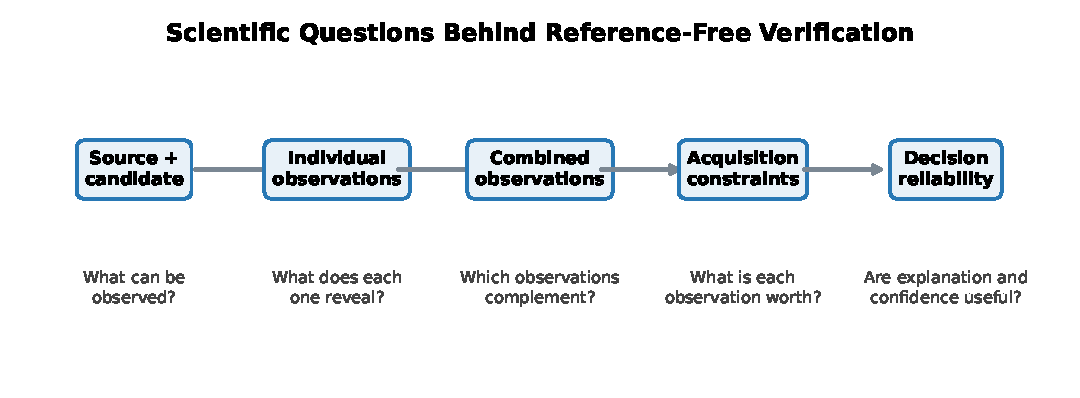
\includegraphics[width=\linewidth]{../figures/verification_study_questions.pdf}}{\fbox{Study-question figure not yet generated}}
  \caption{The investigation begins with questions rather than an assumed hierarchy: what can be observed from a source--candidate pair, what does each observation reveal, how do observations interact, what do they cost, and are the resulting explanations and confidence reliable?}
  \label{fig:study-questions}
\end{figure}

With the practical gap established, the next section positions evidence accumulation relative to existing evaluation and verification techniques; the following problem formulation then defines exactly what is observed.

\section{Related Work}
To understand why another similarity score is insufficient, we first trace what existing evaluation methods can observe and which resources they assume.
Generated-code evaluation spans methods with fundamentally different information requirements. Reference-based similarity methods require a trusted target-language implementation and measure resemblance to that implementation; they therefore address a different inference setting from EviCode and are not treated as baselines in this study. Execution-based evaluation instead requires tests and a runnable environment, and emphasizes functional correctness on observed inputs~\cite{chen2021evaluating,cassano2023multiple,zheng2023codegeex}. Software-testing and repair research further warns that tests are bounded by oracle availability, coverage, adequacy, and plausible-but-wrong outputs~\cite{barr2015oracle,inozemtseva2014coverage,jia2011mutation,yoo2012regression,legoues2012genprog,just2014defects4j,monperrus2018automatic}.

Reference-free QE provides the closest task-level precedent. WMT QE evaluates systems that predict sentence- or word-level translation quality from source and hypothesis without seeing a reference~\cite{fonseca2019wmtqe,blain2023wmtqe}. OpenKiwi packages predictor--estimator and related neural QE systems at both granularities~\cite{kepler2019openkiwi}; TransQuest fine-tunes cross-lingual transformers for sentence-level QE~\cite{ranasinghe2020transquest}; and COMET-QE/CometKiwi combines multilingual COMET representations with predictor--estimator, word-level, and explanation objectives~\cite{rei2022cometkiwi,rei2023scalingcometkiwi}. These approaches establish that useful quality signals can be learned without a target reference, including finer-grained error predictions. EviCode transfers the resource assumption, not the natural-language model: it operates on executable programs; measures explicit syntax, structure, control flow, operators, identifier roles, data flow, APIs, complexity, and execution; normalizes those observations across programming languages; and studies semantic observability, acquisition cost, calibration, and complementarity. Natural-language QE systems are therefore conceptual task relatives rather than direct code-verification baselines.

Program translation and code-intelligence work motivates the need for reference-free verification. TransCoder, CodeBERT, GraphCodeBERT, CodeT5, CodeXGLUE, and related representation-learning systems show that programs expose lexical, syntactic, structural, and semantic views~\cite{roziere2020transcoder,feng2020codebert,guo2021graphcodebert,wang2021codet5,lu2021codexglue,alon2019code2vec,mou2016tbcnn,allamanis2018survey}. Cross-language clone detection and code search study similarity~\cite{sajnani2016sourcerercc,jiang2007deckard,roy2009comparison}, while static analysis and verification provide stronger but more assumption-heavy reasoning tools~\cite{cousot1977abstract,hind2001pointer,tip1995slicing,necula1997proof,leino2010dafny}. EviCode differs by treating these observations as measurable evidence sources for generated-code verification, not as a single scalar metric or a claim of formal equivalence.

The closest gap is therefore not another leaderboard metric. It is a systematic account of what each evidence source observes, what it misses, which sources are redundant, and whether confidence remains calibrated under language and dataset shift~\cite{guo2017calibration}.

\section{Problem and Formalization}
The resource gap motivates a precise question: what does it mean to compare a source program with a generated candidate when neither a target-language reference nor complete behavior is observable?
Let $x$ be a source program and $y$ be a generated candidate in a target language. Semantic verification asks whether $y$ preserves the intended behavior of $x$ for the task under consideration. This question is related to, but distinct from, textual similarity, parseability, compilation, and passing tests. Each of those observations is evidence about correctness; none is the definition of correctness by itself.

We use the running example in Table~\ref{tab:running-example} throughout the paper. The Python source computes addition. Candidate A is a Java translation that changes addition to subtraction; Candidate B reverses operand order but preserves integer addition. The pair is deliberately simple because it isolates the central difficulty: A resembles the source closely but is wrong, whereas B differs in token order but is correct.

\begin{table}[!htbp]
\centering
\caption{Running example used to explain how evidence sources distinguish resemblance from semantic consistency.}
\label{tab:running-example}
\footnotesize
\resizebox{\columnwidth}{!}{%
\begin{tabular}{@{}lll@{}}
\toprule
Program & Core expression & Semantic status \\
\midrule
Python source & \texttt{return a + b} & intended behavior \\
Candidate A & \texttt{return a - b;} & incorrect operator \\
Candidate B & \texttt{return b + a;} & equivalent for integers \\
\bottomrule
\end{tabular}
}
\vspace{0.5em}
\end{table}

The formal target is $c(x,y)=1$ when $x$ and $y$ induce the same task-relevant behavior over domain $\mathcal{D}$, but $\mathcal{D}$ is rarely fully observable. EviCode therefore studies an evidence vector $E(x,y)=[e_1(x,y),\ldots,e_k(x,y)]$ and a calibrated confidence $f_\theta(E)=P_\theta(c=1\mid E)$. We measure evidence usefulness through mutual information $I(e_i;c)$, complementarity $\Delta(A,B)=Q(A\cup B)-\max(Q(A),Q(B))$, ablations, calibration error, and cost-aware execution budgets $E_b=E_{\mathrm{static}}\cup E_{\mathrm{exec}}^b$.

EviCode organizes evidence as $\mathcal{H}=\langle L,S,R,B,D\rangle$: lexical proxies, syntactic validity, structural evidence, static behavioral evidence, and dynamic execution. The static extractor maps each program to a language-normalized profile $\phi(p)=[c(p),s(p),o(p),i(p),d(p),q(p)]$ covering control flow, structure, operator families, identifier roles, approximate data flow, complexity, and validity. Scalar properties use ratio similarity and histogram properties use cosine similarity. Thus Python and Java snippets are compared through normalized program properties, not raw abstract-syntax-tree (AST) node vocabularies. Execution evidence remains separate because it observes behavior on sampled inputs.

The central hypothesis is not that static evidence proves equivalence. Different sources reduce different uncertainties: lexical and raw AST proxies support cheap plausibility, syntax filters unusable candidates, static semantic evidence exposes operators, application programming interfaces (APIs), roles, and value movement, and tests provide the strongest available observation when they exist.

The formalization identifies what must be compared but not yet how Python and Java become comparable. The next subsection introduces the paper's central representation and explains the uncertainty addressed by every evidence family.

\subsection{Language-Normalized Evidence Representation}
\textbf{Definition.} Let $g_\ell:P_\ell\rightarrow\mathcal{Z}$ map a program written in language $\ell$ to a shared property space $\mathcal{Z}$. An observation is \emph{language-normalized} when (i) parsing is performed with a language-specific front end, (ii) parser-specific constructs are mapped to a shared program concept, (iii) quantities are compared with a scale-aware function, and (iv) the observation's unsupported semantics are stated explicitly. EviCode instantiates scalar comparison as $r(a,b)=\min(a,b)/\max(a,b)$ (with equality for two zeros) and distributional comparison as cosine similarity. Consequently, one branch in Python and one branch in Java agree as instances of the shared concept \emph{conditional control}, whereas Python and Java AST node names are never equated directly.

These criteria provide comparability, not invariance under all semantics-preserving transformations. Formatting and parser vocabulary should not change a normalized observation, but refactoring, library substitution, type behavior, or language idioms can. EviCode first extracts a profile from each program in its own language, then compares corresponding properties: branches, loops, returns, nesting, cyclomatic complexity, operator families, statement distributions, identifier-role distributions, and approximate read/write behavior. Raw token and AST overlap are retained only as explicitly labeled weak proxies because they do not satisfy the same semantic interpretability criterion.

\textbf{Intuition and example.} Table~\ref{tab:normalized-example} compares a Python maximum function with \texttt{if a > b: return a; else: return b} and a Java translation with \texttt{if(a>b)\{return a;\} return b;}. Their syntax differs, but both profiles contain approximately one branch, two returns, zero loops, maximum nesting one, cyclomatic complexity two, and one comparison operator. These properties can be compared directly because ``branch'' and ``comparison'' denote program concepts rather than parser-specific symbols. Formatting, braces, indentation, keyword spelling, and raw AST node labels are intentionally ignored by this normalized comparison.

\begin{table}[!t]
\centering
\footnotesize
\caption{A Python and Java maximum function have different syntax but approximately the same language-normalized semantic profile.}
\label{tab:normalized-example}
\begin{tabular}{@{}lcc@{}}
\toprule
Property & Python & Java \\
\midrule
Branches & 1 & 1 \\
Returns & 2 & 2 \\
Loops & 0 & 0 \\
Maximum nesting & 1 & 1 \\
Cyclomatic complexity & 2 & 2 \\
Comparison operators & 1 & 1 \\
\bottomrule
\end{tabular}
\end{table}

The scientific interpretation is that EviCode compares semantic program properties rather than language syntax. Normalization does not make the properties complete semantics: two programs can share every listed count and still compute different values. It makes partial observations commensurable, while leaving their limitations visible.

\paragraph{Lexical evidence: What symbols were used?}
\textbf{Definition and intuition:} token overlap, edit similarity, and length ratio measure surface correspondence; shared symbols can indicate that a translation retained task vocabulary. In the running example, both candidates retain \texttt{a}, \texttt{b}, and \texttt{return}, so lexical evidence considers both plausible. \textbf{Interpretation:} it reduces uncertainty about gross topical or signature mismatch. \textbf{Limitation:} it ignores meaning; Candidate A remains lexically close despite replacing \texttt{+} with \texttt{-}, and renamed variables can lower overlap without changing behavior.

\paragraph{Syntax validity: Can the program be parsed?}
\textbf{Definition and intuition:} each program is parsed with its own language parser, and validity is compared as a boolean property. Both running candidates parse, so syntax removes the possibility of malformed Java but cannot distinguish them. \textbf{Interpretation:} it removes grammatical uncertainty without comparing Python productions to Java productions. \textbf{Limitation:} a well-formed program may not compile or behave correctly.

\paragraph{Program structure: Is the code organized similarly?}
\textbf{Definition and intuition:} normalized tree depth, statement distributions, function/class counts, and broad AST shape summarize organization. Both running candidates have one method and one return expression, so structure supports alignment. \textbf{Interpretation:} it reduces uncertainty that the candidate implements a wholly different organizational form. \textbf{Limitation:} shape can remain unchanged when one token reverses the computation; raw AST-node similarity is therefore treated as a weak cross-language proxy.

\paragraph{Control flow: Can it follow similar execution paths?}
\textbf{Definition and intuition:} branch, loop, return, exception, nesting, and normalized control-flow-graph (CFG) count profiles approximate possible execution paths. The two straight-line running candidates have the same control profile. \textbf{Interpretation:} control agreement removes uncertainty about missing branches, extra loops, or changed termination structure. \textbf{Limitation:} identical paths can execute different expressions, and count-based profiles do not establish path correspondence.

\paragraph{Operator evidence: Does it perform the same local computation?}
\textbf{Definition and intuition:} arithmetic, comparison, logical, and assignment operators are mapped into shared families. Candidate A changes the source's arithmetic operation from addition to subtraction and therefore weakens operator evidence; Candidate B preserves addition despite reversing operands. \textbf{Interpretation:} this family removes uncertainty about local computation that broad structure misses. \textbf{Limitation:} matching histograms do not capture operand order, overloads, numeric types, or context-dependent operator behavior.

\paragraph{Identifier roles: Do variables keep their responsibilities?}
\textbf{Definition and intuition:} the extractor distinguishes declarations, assignments, and calls and compares both role counts and rough role distributions. Names may change across languages, but responsibilities such as ``parameter used in the returned expression'' often remain. Both running candidates preserve the two parameter roles; a candidate that overwrites one parameter would not. \textbf{Interpretation:} role evidence reduces uncertainty about which values participate in computation. \textbf{Limitation:} the analysis is approximate; raw name overlap remains language-sensitive, and role counts cannot prove that the correct value occupies each role.

\paragraph{Data flow: Are values propagated similarly?}
\textbf{Definition and intuition:} approximate definition--use pairs, assignment density, and read/write ratios summarize value propagation. For the running example, both parameters flow into the return expression, whereas a candidate returning only \texttt{a} would lose one dependency. \textbf{Interpretation:} data-flow evidence reduces uncertainty about whether required inputs reach outputs. \textbf{Limitation:} the implementation is name- and pattern-based rather than path-sensitive analysis; aliasing, heap state, and interprocedural flow are intentionally ignored.

\paragraph{API evidence: Does it invoke compatible operations?}
\textbf{Definition and intuition:} call tokens, imports, and API overlap indicate whether a candidate invokes a compatible library operation. A translation using a nonexistent \texttt{Math.plus(a,b)} would be suspicious even if its intended arithmetic is clear. \textbf{Interpretation:} API evidence reduces uncertainty about target-language library and call consistency. \textbf{Limitation:} APIs are inherently language-specific, so this family is a weak proxy across languages; equivalent libraries may have unrelated names, and matching names do not guarantee matching contracts.

\paragraph{Complexity: Does it contain a similar amount of logic?}
\textbf{Definition and intuition:} cyclomatic complexity, nesting depth, and statement/expression density summarize computational shape. The straight-line source and both candidates have similar low complexity. \textbf{Interpretation:} large disagreement can expose omitted cases or unnecessary control machinery. \textbf{Limitation:} complexity describes amount and shape of logic, not correctness; equally complex programs can implement unrelated functions.

\paragraph{Execution: Does it behave correctly on tested inputs?}
\textbf{Definition and intuition:} example or full tests run the candidate and observe outputs. Inputs such as $(3,2)$ immediately separate Candidate A ($1$) from Candidate B ($5$). \textbf{Interpretation:} execution removes uncertainty about behavior on tested inputs and therefore occupies the highest ladder level. \textbf{Limitation:} untested inputs remain unknown, and execution requires tests, dependencies, isolation, and runtimes.

Together, these families form an evidence vocabulary: early levels reject implausible form, middle levels expose program obligations, and tests observe selected outcomes. This vocabulary motivates the research questions below, which ask not whether one new classifier wins, but which observations are informative, complementary, affordable, explanatory, and calibrated.

\section{Research Questions}
EviCode asks four research questions. They form one evidence argument: first measure what each source knows, then test whether sources add non-redundant information, determine what richer observations cost, and finally examine whether the resulting decisions are interpretable and calibrated.

\textbf{RQ1: Informativeness.} Which evidence sources are individually most informative for semantic correctness?

\textbf{RQ2: Complementarity.} Which evidence sources add value when combined, and which are redundant?

\textbf{RQ3: Execution budget and cost.} How does verification change as dynamic evidence moves from unavailable to partial to full, and what infrastructure cost does each evidence source require?

\textbf{RQ4: Interpretability and reliability.} Can decomposed evidence support actionable failure explanations, and does fused confidence retain probabilistic meaning on held-out data?

Answering these questions requires preserving evidence sources long enough to analyze them separately. The architecture therefore separates extraction, aggregation, and reporting rather than hiding them inside one learned representation.

\section{Architecture}
The EviCode pipeline separates evidence extraction from confidence estimation. Here, \emph{evidence fusion} simply means combining several partial observations into one confidence while retaining their individual identities. As shown in Figure~\ref{fig:pipeline}, a generated candidate is not sent directly to a black-box classifier. Specialized extractors answer separate questions, the analysis instrument combines their answers, and the report names the strongest and weakest sources. Trust decisions can therefore expose the observations behind them.

\begin{figure*}[!t]
  \centering
  \IfFileExists{../figures/pipeline.pdf}{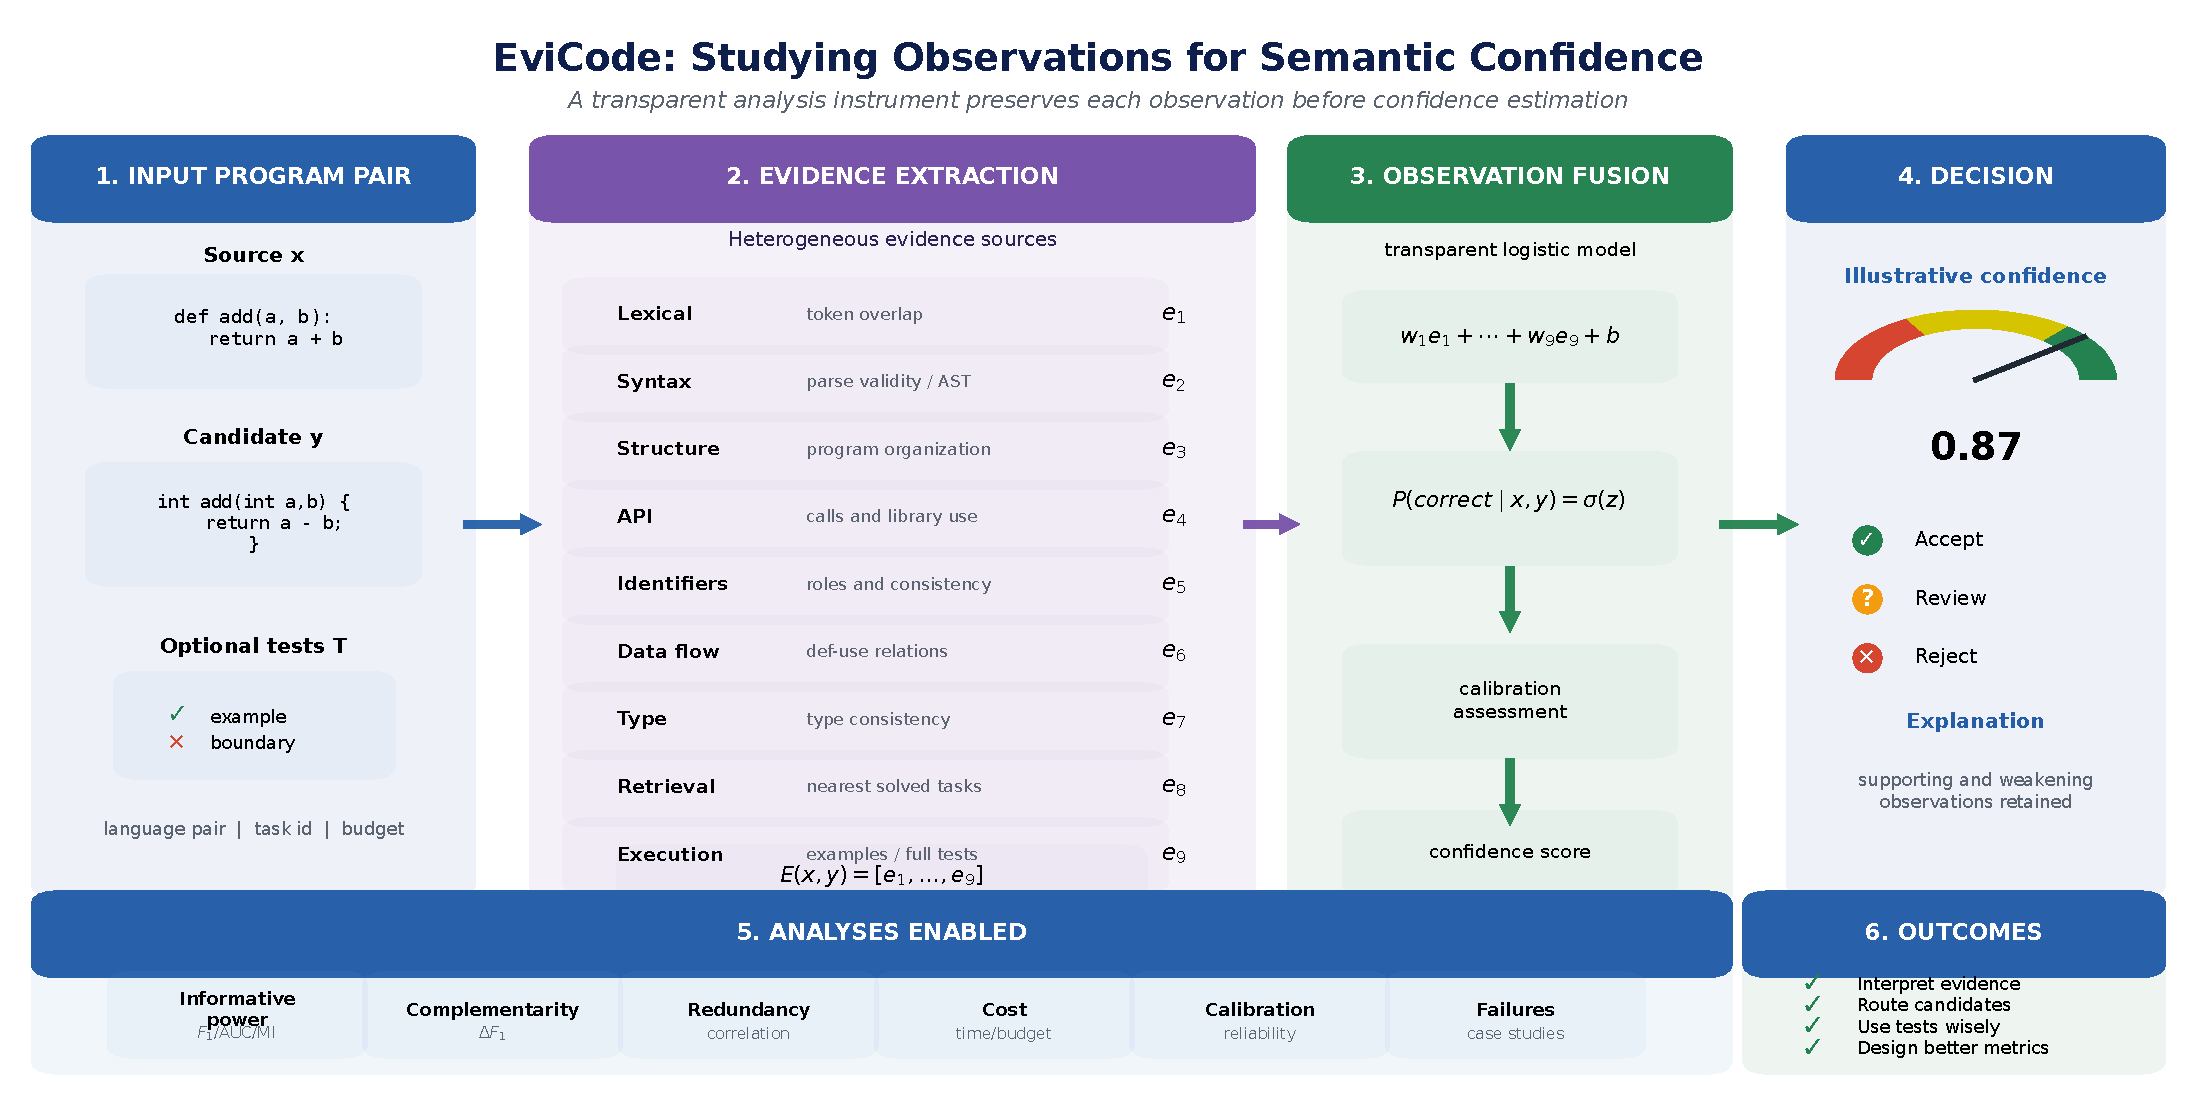
\includegraphics[width=0.96\textwidth]{../figures/pipeline.pdf}}{\fbox{EviCode workflow not found}}
  \caption{End-to-end analysis workflow. A source--candidate pair is converted into explicit observations, a transparent logistic model estimates confidence, and calibration is evaluated rather than assumed. Preserving observation identities enables the information, complementarity, cost, and failure analyses used in this study.}
  \label{fig:pipeline}
\end{figure*}

The pipeline in Figure~\ref{fig:pipeline} matters because it makes the verifier auditable. A monolithic score can be high for several incompatible reasons: lexical overlap, parse validity, structural similarity, successful tests, or dataset-specific correlations. EviCode preserves those reasons as separate evidence channels before fusion, which makes it possible to ask whether the verifier is relying on behavior, surface form, or an artifact of the benchmark.

The architecture defines what is observable; the experimental design must next ensure that apparent evidence value is not produced by task leakage, class imbalance, or one favorable operating threshold.

\section{Experimental Design}
\subsection{Datasets}
The main study uses HumanEval-X for Python, Java, and JavaScript. For each of 164 tasks, EviCode constructs directed source-target verification examples across the three languages. Positive examples pair programs for the same task. Negative examples are produced through task mismatching and controlled target mutation. This yields 2,952 verification examples: 984 positives and 1,968 negatives.

\IfFileExists{../tables/dataset_statistics.tex}{\begin{table}[!htbp]
\centering
\small
\begin{tabular}{ll}
\toprule
Statistic & Value \\
\midrule
Languages & java, js, python \\
Problems & 164 \\
Verification pairs & 2952 \\
Positive pairs & 984 \\
Negative pairs & 1968 \\
Avg. source chars & 322 \\
Avg. target chars & 323 \\
\bottomrule
\end{tabular}
\vspace{0.5em}
\caption{HumanEval-X verification examples used in the main study, including directed source-target pairs and positive/negative correctness labels.}
\label{tab:dataset-statistics}
\end{table}
}{}
\IfFileExists{../tables/evidence_taxonomy.tex}{\begin{table}[!htbp]
\centering
\scriptsize
\begin{tabular}{lll}
\toprule
Evidence & Category & Cost \\
\midrule
Token overlap & Weak-proxy & low \\
Edit similarity & Weak-proxy & low \\
Length ratio & Lexical & low \\
Parse validity & Syntactic & low \\
AST node similarity & Weak-proxy & medium \\
AST depth similarity & Normalized-structure & medium \\
AST shape similarity & Normalized-structure & medium \\
Control flow & Normalized-control & low \\
Nesting depth & Normalized-control & low \\
Condition/operator patterns & Normalized-operator & low \\
API overlap & Weak-proxy & low \\
API mismatch & Weak-proxy & low \\
\bottomrule
\end{tabular}
\vspace{0.5em}
\caption{EviCode evidence taxonomy, organized by source type so that syntax, structure, API, identifier, retrieval, and execution evidence can be studied separately.}
\label{tab:evidence-taxonomy}
\end{table}
}{}

The dataset scale in Table~\ref{tab:dataset-statistics} supports a controlled empirical study rather than a broad benchmark claim. The 2,952 examples are large enough for grouped train/test evaluation and paired statistical tests, while the 164 underlying problems keep the setting interpretable enough for qualitative disagreement analysis. The 1:2 positive-to-negative balance also matters: accuracy alone would be misleading, so the study emphasizes F1, AUC, calibration, and paired comparisons.

The taxonomy is included to answer a practical question: what kinds of uncertainty can be observed before tests run? Table~\ref{tab:evidence-taxonomy} spans low-cost lexical features, parse and AST evidence, control-flow and operator patterns, and API-level evidence. Most static sources are cheap, but each exposes a different failure surface, allowing malformed, API-incoherent, and structurally plausible but computationally suspicious candidates to be distinguished.

\subsection{Models, Splits, and Statistics}
Experiments use grouped problem-level train/test splitting so all directed pairs for a held-out task remain in the test partition. We intentionally use logistic regression as a transparent linear analysis instrument because the objective is to study observations rather than maximize predictive performance with an opaque learner. F1 measures accept/reject quality, receiver operating characteristic AUC (ROC-AUC) measures ranking, bootstrap intervals and McNemar tests quantify uncertainty, mutual information and coefficients characterize evidence use, and calibration measures whether confidence retains probabilistic meaning.

\subsection{Evaluation Metrics}
Evaluation separates decisions, ranking, probability quality, information, and explanation. F1 summarizes the balance between accepting correct candidates and avoiding incorrect acceptance. ROC-AUC asks how often a randomly chosen correct candidate ranks above an incorrect one, independent of one threshold; precision--recall AUC (PR-AUC) focuses on the quality of retrieved correct candidates. Calibration asks whether stated confidence matches observed correctness, using Brier score, expected calibration error, and reliability bins. Mutual information measures how much knowing one observation reduces uncertainty about the label. Coefficients and feature attributions then ask how the model uses observations together. Bootstrap intervals and paired McNemar tests quantify sampling uncertainty and decision disagreement. Source--candidate similarities and execution are evaluated as evidence signals, not assumed to define equivalence.

With these controls in place, the results follow the same progression as the ladder: individual information, complementary accumulation, acquisition cost, diagnostic value, and calibrated confidence.

\section{Results and Analysis}
This section follows the questions a reader would face when acquiring verification evidence. First, how much can be learned before running a program? Second, do different observations add new information or repeat one another? Third, when is execution worth its cost? Fourth, can the resulting decision explain what deserves attention, and can its confidence be interpreted? Each subsection moves from the experiment to the observation, its cause, and its broader implication.

\subsection{RQ1: Which Evidence Is Informative?}
\subsubsection{Evidence Strength Follows Observability}
We begin by asking how verification changes when observation moves from program properties to tested outcomes. Enriched static evidence reaches F1 0.558, whereas dynamic evidence reaches F1 0.904 (Table~\ref{tab:evidence-group-results}). A 34.6-point gap is large: it marks a change in what is knowable, not a small improvement from another feature. Static evidence estimates plausibility from validity, control, operators, roles, calls, and data-flow proxies; execution observes consequences on concrete inputs. Behavioral observation therefore resolves uncertainty that program form alone leaves open.

Static observations should not be dismissed simply because they classify poorly at one threshold. Without a reference or execution, they rank a randomly selected correct translation above an incorrect one about 80\% of the time (AUC 0.801). Ranking only requires relative plausibility; reliable acceptance requires a boundary that static form cannot supply. Generated programs preserve enough structure, control, operators, and roles for prioritization, while tested behavior supplies information for acceptance under the available tests. Static observations are therefore suited to ordering, early rejection, and allocating execution or review.

\subsubsection{Static Evidence Supports Prioritization}
The gap between F1 and AUC is itself informative. Static evidence has modest thresholded F1 but strong ranking ability, which means it often orders candidates sensibly even when a single accept/reject boundary is unreliable. This distinction separates two roles for evidence. Behavior-based evidence supports acceptance decisions when tests are available and meaningful, but remains bounded by those tests. Representation-based evidence is suitable for prioritization because it cheaply estimates plausibility. In practical terms, static evidence can separate hopeless candidates from plausible ones, route suspicious translations to execution or repair, and explain why a candidate deserves scrutiny.

The individual evidence groups clarify this point. Lexical-only and syntactic-only evidence both have F1 0.000 in Table~\ref{tab:evidence-group-results}, with AUC 0.552 and 0.589 respectively. This does not mean lexical or syntax evidence is useless. It means that, by themselves, these signals behave more like gates or weak rankers than final classifiers. Once many candidates share similar surface plausibility or parse successfully, neither source can separate semantic correctness at a fixed threshold. The stronger static result appears only after many static observations are fused: the static verifier reaches F1 0.558 and AUC 0.801. Thus, the important lesson is that cheap static evidence becomes useful through aggregation and ranking, not through any single lexical or syntactic cue.

\subsubsection{Fusion Improves Confidence Structure}
Fusion confirms that static evidence mainly refines confidence once behavior has been observed. Static plus example execution reaches F1 0.859, static plus full execution reaches F1 0.865, and the all-evidence model reaches F1 0.869 with the strongest AUC, 0.959. The thresholded F1 values change only modestly across execution-heavy configurations because execution already contains most of the decision-relevant behavioral information. The larger AUC effect tells a different story: static evidence improves confidence ordering among candidates whose execution evidence may be similar, partial, or noisy.

This is an important design insight. Evidence fusion should not be judged only by whether it beats execution at one operating threshold. When F1 barely changes but AUC improves, the verifier has become better at ranking uncertainty rather than simply producing more positive labels. That is useful for downstream systems that must decide which candidates to execute fully, repair, accept with caution, or send to a developer. Static evidence is therefore complementary to execution primarily as confidence refinement and explanation, not as a replacement for behavioral information.

\IfFileExists{../tables/evidence_group_results.tex}{\begin{table}[!htbp]
\centering
\scriptsize
\begin{tabular}{lrrrr}
\toprule
Group & Acc. & F1 & AUC & Feat. \\
\midrule
Lexical & 0.667 & 0.000 & 0.552 & 1 \\
Syntactic & 0.667 & 0.000 & 0.589 & 1 \\
Structural & 0.681 & 0.364 & 0.653 & 24 \\
SemStatic & 0.670 & 0.252 & 0.717 & 12 \\
Dynamic & 0.929 & 0.904 & 0.947 & 2 \\
Static & 0.743 & 0.558 & 0.801 & 45 \\
Static+Ex. & 0.900 & 0.859 & 0.933 & 46 \\
Static+Full & 0.906 & 0.865 & 0.959 & 46 \\
All & 0.908 & 0.869 & 0.959 & 47 \\
\bottomrule
\end{tabular}
\vspace{0.5em}
\caption{Held-out HumanEval-X verification performance for individual evidence groups and fused combinations.}
\label{tab:evidence-group-results}
\end{table}
}{}
\IfFileExists{../tables/evidence_informativeness.tex}{\begin{table}[!htbp]
\centering
\scriptsize
\begin{tabular}{llrr}
\toprule
Evidence & Category & AUC & MI \\
\midrule
Full execution & Dynamic & 0.934 & 0.411 \\
Example execution & Dynamic & 0.913 & 0.361 \\
AST node similarity & Weak-proxy & 0.550 & 0.109 \\
Token overlap & Weak-proxy & 0.739 & 0.097 \\
Condition/operator patterns & Normalized-operator & 0.633 & 0.069 \\
Identifier overlap & Semantic-static & 0.709 & 0.053 \\
\bottomrule
\end{tabular}
\vspace{0.5em}
\caption{Evidence features with the highest individual mutual information with the HumanEval-X correctness label.}
\label{tab:evidence-informativeness}
\end{table}
}{}
\IfFileExists{../tables/evidence_hierarchy.tex}{\begin{table}[!htbp]
\centering
\scriptsize
\begin{tabular}{lrrrr}
\toprule
Level & Feat. & F1 & AUC & Delta F1 \\
\midrule
Weak proxy & 8 & 0.461 & 0.805 & 0.461 \\
Program & 9 & 0.460 & 0.805 & -0.001 \\
Control/structure & 31 & 0.478 & 0.806 & 0.018 \\
Semantic static & 45 & 0.558 & 0.801 & 0.081 \\
Dynamic & 47 & 0.869 & 0.959 & 0.311 \\
\bottomrule
\end{tabular}
\vspace{0.5em}
\caption{Incremental predictive value as evidence groups are added from lexical/static features toward dynamic execution evidence.}
\label{tab:evidence-hierarchy}
\end{table}
}{}
\FloatBarrier

\subsubsection{Useful Static Evidence Exposes Failure Modes}
To learn which individual observations deserve attention, we compare how much each reduces uncertainty about correctness. Full and example execution have mutual information (MI) of 0.411 and 0.361, while the strongest static observations are much smaller: raw AST similarity at 0.109 and token overlap at 0.097 (Table~\ref{tab:evidence-informativeness}). Execution therefore carries roughly four times as much individual label information as the strongest static feature. AST and token evidence still help with plausibility, but their small values explain why they cannot stand in for behavior.

The static ordering is more interesting than a flat ranking. Token overlap has lower MI than raw AST node similarity, but much higher AUC, 0.739 versus 0.550. This mismatch shows that mutual information and ranking ability capture different aspects of evidence. Raw AST similarity can be informative in aggregate because correct and incorrect candidates often differ in construction, but it is weak as a ranker across languages because Python and Java grammars expose different node vocabularies. It captures construction resemblance, not semantic correctness. Identifier overlap has lower MI, 0.053, but respectable AUC 0.709, suggesting that names can help rank plausibility even when they are not a decisive source by themselves.

Operator-pattern evidence provides the clearest design lesson. Its MI, 0.069, is below raw AST similarity, but its AUC, 0.633, is more semantically meaningful because small operator or predicate changes can completely alter behavior while preserving the surrounding syntactic form. This explains why high-level syntax resemblance can be less defensible than language-normalized behavioral primitives. Static evidence should therefore be selected for the failure modes it exposes: weak proxies for cheap plausibility, normalized control profiles for execution-shape drift, identifier-role distributions for value responsibility, data-flow proxies for movement of values, and operator families for local computation changes.

\subsubsection{Verification Behaves Like Progressive Uncertainty Reduction}
The cumulative comparison asks where each step of the ladder changes verification. Weak lexical, syntactic, and cross-language proxies reach F1 0.461 and AUC 0.805. Adding coarse program counts changes little, indicating redundancy. Control and structure increase F1 to 0.478, and complete static semantic evidence reaches 0.558. The largest transition occurs when execution enters: F1 rises to 0.869 and AUC to 0.959, a gain of 0.311 over static evidence (Table~\ref{tab:evidence-hierarchy} and Figure~\ref{fig:evidence-hierarchy}).

The shape matters more than any one value. Static evidence reduces uncertainty gradually, then execution creates a qualitative transition. Control and structure add only 0.018 F1 because validity and coarse form already capture related information. Operators, identifier roles, calls, and data flow add 0.081, enough to improve diagnosis but not replace tests. Verification is therefore progressive observation rather than simple feature accumulation.

Each position follows from its observation boundary. Raw tokens constrain intent only through shared symbols. Parsing removes grammatically impossible candidates but says little about task behavior. Structure and control flow constrain organization and possible execution shapes without resolving computations on those paths. Operators and identifier roles expose local transformations and value responsibilities; data-flow proxies connect those observations into approximate value propagation. Execution is highest because it observes consequences, although only over tested inputs. An upward step therefore means that fewer semantically distinct programs remain observationally indistinguishable, not merely that a classifier scored better.

\begin{figure}[!htbp]
  \centering
  \IfFileExists{../figures/information_gain_hierarchy.pdf}{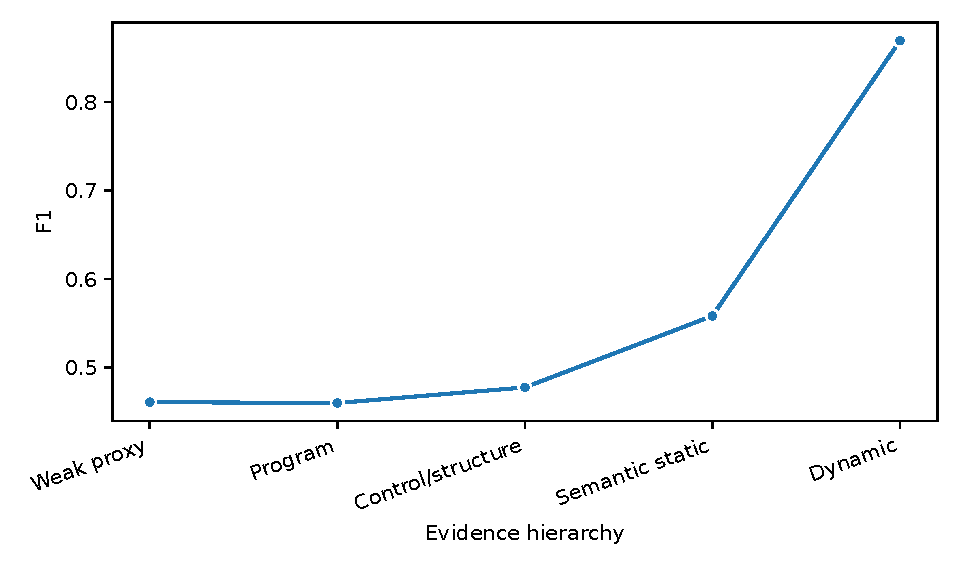
\includegraphics[width=0.88\linewidth]{../figures/information_gain_hierarchy.pdf}}{\fbox{Hierarchy figure not yet generated}}
  \caption{Cumulative evidence performance across the ladder. Small static gains indicate overlapping partial observations; the abrupt execution gain identifies tested behavior as information that structure alone cannot recover.}
  \label{fig:evidence-hierarchy}
\end{figure}

\subsubsection{Implications}
Together, these results support the view that semantic verification is an evidence accumulation process rather than a similarity scoring problem. Static evidence cannot certify correctness, but it substantially reduces uncertainty and enables effective prioritization before tests are available. Execution introduces a qualitative shift because it observes behavior rather than approximating it. Different static evidence sources matter because they expose different failure modes, making their combination more useful than any individual static metric. The proposed evidence ladder is therefore not only a conceptual organization; the experiments recover the same progression empirically, from surface plausibility to validity, from validity to program obligations, and from obligations to observed behavior.

This interpretation also clarifies what future verification systems should optimize. If execution is unavailable, the objective is to maximize the usefulness of early evidence for routing and diagnosis. If execution is available, the objective shifts toward calibration, explanation, and confidence refinement. EviCode keeps both regimes visible: it can report not only whether execution succeeded, but also whether the candidate appeared syntactically valid, structurally aligned, API-consistent, and behaviorally plausible before tests were considered.

The broader implication of RQ1 is that usefulness is governed by what an observation can see. Surface and structural observations can rank and explain candidates, while tested outcomes answer a stronger question. Yet no static observation is decisive alone. This naturally motivates RQ2: can observations become more useful by complementing one another?

\subsection{RQ2: Which Evidence Is Complementary?}
\subsubsection{Complementarity Comes From Different Failure Surfaces}
The next question is whether multiple observations reveal different facts or merely rename the same signal. Combinations containing execution rank candidates best: static plus full execution reaches F1 0.865 and AUC 0.959, while static plus example execution reaches F1 0.859 and AUC 0.933 (Table~\ref{tab:evidence-complementarity}). Static families are weaker, but syntax, control, operators, roles, and data flow expose different failure surfaces. Complementarity therefore comes from distinct ways to be wrong, not from accumulating more feature columns.

This changes how static evidence should be interpreted. It is not a weaker substitute for execution; it is a filter and explanation layer. High static evidence followed by failed tests identifies a behavioral fault hidden behind plausible form, while low static evidence can route a candidate to repair before expensive testing. Evidence integration therefore combines observations whose disagreements reveal something about correctness, rather than maximizing the number of signals.

\IfFileExists{../tables/evidence_complementarity.tex}{\begin{table}[!htbp]
\centering
\scriptsize
\begin{tabular}{lrr}
\toprule
Combination & F1 & AUC \\
\midrule
static\_plus\_full\_execution & 0.865 & 0.959 \\
static\_plus\_example\_execution & 0.859 & 0.933 \\
syntactic\_plus\_weak\_proxy & 0.455 & 0.807 \\
normalized\_program\_plus\_weak\_proxy & 0.455 & 0.807 \\
normalized\_control\_plus\_normalized\_program & 0.437 & 0.716 \\
normalized\_control\_plus\_syntactic & 0.437 & 0.716 \\
normalized\_program\_plus\_semantic\_static & 0.410 & 0.812 \\
semantic\_static\_plus\_syntactic & 0.410 & 0.812 \\
\bottomrule
\end{tabular}
\vspace{0.5em}
\caption{Best pairwise and fused evidence-group combinations on HumanEval-X, used to identify complementary sources beyond single evidence families.}
\label{tab:evidence-complementarity}
\end{table}
}{}

The complementarity results are most important as a confidence-structure result rather than a thresholded leaderboard. Adding static evidence to full execution only slightly changes F1, but it improves AUC because the fused score can rank candidates more finely than a binary execution outcome. Conversely, weak static sources can matter when fused with other static gates, because neither source is sufficient alone. This supports the paper's central claim: evidence sources are not interchangeable metrics; they interact according to what uncertainty each source reduces.

\subsubsection{Ablation Reveals Which Static Observations Matter}
The ablation and importance results make complementarity concrete. Full execution has the largest coefficient magnitude, 3.265, as expected. Below execution, token overlap and operator patterns have the strongest influence, 0.745 and 0.714. Function and CFG counts follow, while broad AST similarity matters less. Richer representation is therefore not automatically closer to meaning: local changes to operators, predicates, APIs, or value roles can preserve the surrounding tree. Observations of computation deserve priority over structural sophistication alone.

The leave-one-out results therefore support a stronger claim than ``structure helps.'' Removing reliability evidence lowers static F1 from 0.558 to 0.436, showing that validity-related signals are a central part of static triage. Removing behavioral evidence lowers F1 to 0.496, and removing operator-pattern similarity alone lowers it to 0.499, a larger degradation than removing raw AST node similarity, which leaves F1 at 0.548. Removing token overlap leaves F1 at 0.535, confirming that surface evidence remains useful for ranking even though it is not semantic. Removing identifier-role similarity leaves F1 at 0.532, while removing the broader structural family leaves F1 at 0.504. The useful static evidence is not simply more structure; it is evidence that moves closer to program obligations: validity, operators, APIs, and value roles.

\subsubsection{Conditional and Marginal Importance}
When correlated observations coexist, a standalone score cannot reveal which ones the fitted model actually uses. SHapley Additive exPlanations (SHAP) addresses this problem by assigning each feature a contribution to the model's prediction relative to an average case. Table~\ref{tab:shap-comparison} and Figure~\ref{fig:shap-importance} compare that contribution with standardized coefficients and mutual information, which measures how informative a feature is by itself. SHAP and coefficients agree strongly ($\rho=0.987$), but SHAP and mutual information agree only moderately ($\rho=0.498$). Token overlap ranks first, while operators, complexity, validity, CFG edges, and identifier roles rise under SHAP because the model uses them conditionally with other evidence. These rankings explain model use, not causal importance.

SHAP is intentionally computed for the static model only. Once tests are included, their strong signal dominates prediction and hides how weaker static observations interact. The question here is how static semantic evidence contributes before test outcomes overwhelm it. Full-model SHAP would mostly explain the execution-heavy predictor rather than the static ladder.

\IfFileExists{../tables/shap_comparison.tex}{\begin{table}
\caption{Top static evidence sources by mean absolute SHAP value on the held-out split. SHAP and coefficients measure conditional model use; MI measures marginal label information.}
\label{tab:shap-comparison}
\begin{tabular}{lrrr}
\toprule
Evidence & SHAP & |Coef.| & MI \\
\midrule
Token overlap & 1.009 & 1.346 & 0.122 \\
Condition/operator patterns & 0.523 & 0.563 & 0.066 \\
LN cyclomatic complexity & 0.483 & 0.527 & 0.030 \\
LN syntax validity & 0.483 & 0.746 & 0.045 \\
Parse validity & 0.483 & 0.746 & 0.040 \\
LN CFG edge count & 0.389 & 0.414 & 0.052 \\
LN statement density & 0.290 & 0.338 & 0.000 \\
Identifier role consistency & 0.280 & 0.385 & 0.016 \\
Control flow & 0.262 & 0.318 & 0.043 \\
LN expression distribution & 0.231 & 0.276 & 0.000 \\
\bottomrule
\end{tabular}
\end{table}
}{}

\begin{figure}[!htbp]
  \centering
  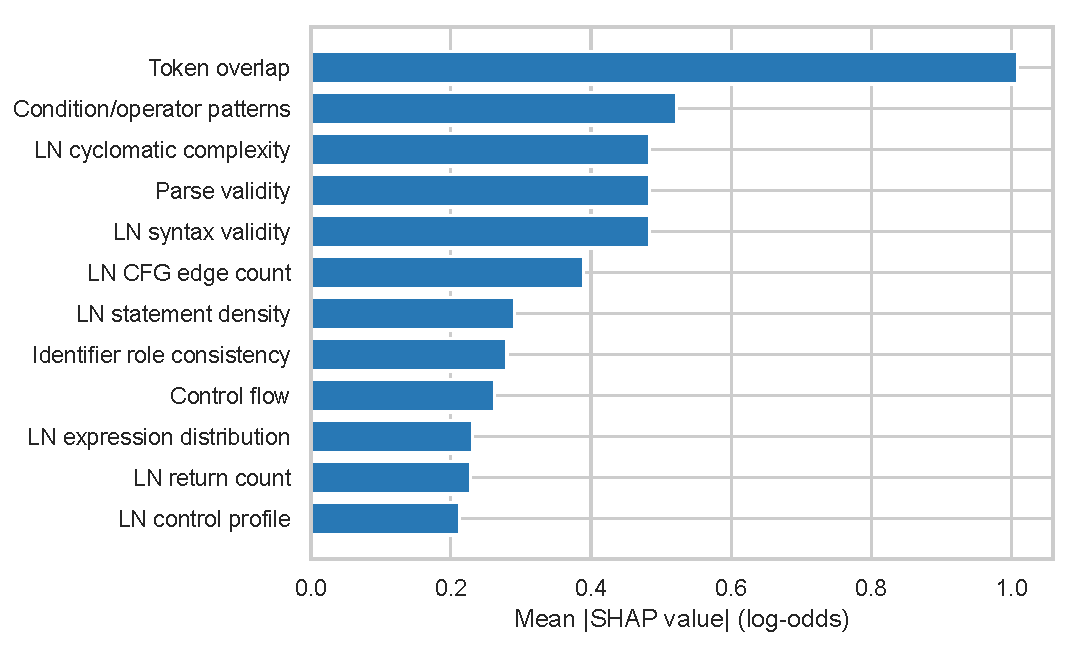
\includegraphics[width=0.92\linewidth]{../figures/shap_feature_importance.pdf}
  \caption{How strongly the static analysis instrument uses each observation. Longer bars mean a larger average change in predicted log-odds; the ranking explains conditional model use before execution dominates, not causal importance.}
  \label{fig:shap-importance}
\end{figure}

Importance rankings alone cannot tell whether two features repeat the same observation. The correlation view below asks where evidence is redundant and where a low-correlation family can contribute a genuinely different warning.

\begin{figure}[!htbp]
  \centering
  \IfFileExists{../figures/evidence_complementarity_heatmap.pdf}{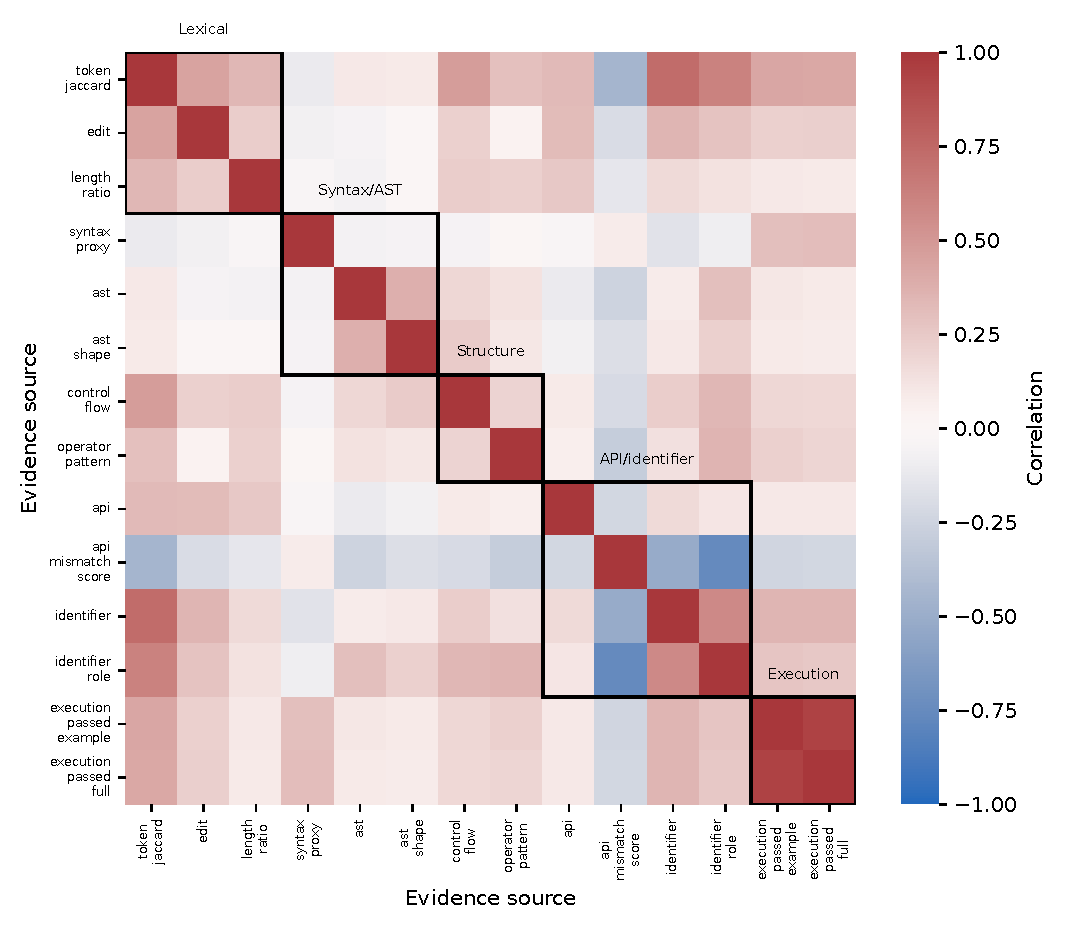
\includegraphics[width=\linewidth]{../figures/evidence_complementarity_heatmap.pdf}}{\fbox{Complementarity heatmap not yet generated}}
  \caption{Which observations repeat one another. High-correlation blocks reveal redundancy; lower-correlation families can add distinct warnings and are therefore more valuable for evidence accumulation.}
  \label{fig:evidence-complementarity}
\end{figure}

\subsubsection{Correlation Separates Redundancy From New Evidence}
The complementarity heatmap in Figure~\ref{fig:evidence-complementarity} acts as a redundancy map. The visible lexical, syntax/AST, API/identifier, and execution clusters show that several features measure related evidence rather than independent facts. Highly correlated feature blocks may improve robustness, but they do not necessarily add new semantic information. Lower-correlation blocks are more useful because they expose different failure surfaces: operator evidence catches small computation changes, API evidence catches target-language misuse, identifier-role evidence catches swapped responsibilities, and execution adjudicates behavior. This is why EviCode evaluates evidence combinations rather than treating all static features as a single undifferentiated representation.

\subsubsection{Implications}
AST similarity is useful for alignment, while operators, APIs, roles, and tests answer questions closer to computation. Verification improves when observations can disagree for meaningful reasons; reporting one aggregate score hides those reasons.

The broader implication of RQ2 is that the best static observations are not necessarily the richest representations. A compact operator or role mismatch can add more than broad structural similarity when it exposes a new way to be wrong. Complementarity explains what should be acquired; RQ3 next asks when its information is worth the computational cost, especially once tests become available.

\subsection{RQ3: How Much Execution Is Necessary?}
\subsubsection{The First Behavioral Signal Changes the Regime}
The cost results show that verification quality cannot be interpreted without evidence availability. HumanEval-X provides example and full test programs but not a normalized list of individual cross-language assertions, so Table~\ref{tab:execution-budget} reports only completed settings: no execution, example-test execution, full-test execution, and their corresponding evidence-fusion configurations. This is a methodological choice. A weak-test curve should measure actual test weakening, not an artifact of inaccessible harness structure.

Within the supported settings, the first dynamic signal has the largest payoff. Static-only verification reaches F1 0.558. Example-test execution reaches F1 0.879, a relative improvement of about 58\% over static-only verification. Full execution reaches F1 0.904, adding a much smaller gain over example execution than the initial move from static evidence to any behavior observation. This does not prove that example tests are sufficient in general; HumanEval-X examples are not a universal coverage model. It shows that the first reliable behavioral observation can change the verification regime: moving from representation to behavior reduces a different kind of uncertainty than adding more static representation.

\IfFileExists{../tables/execution_budget_results.tex}{\begin{table}[!htbp]
\centering
\scriptsize
\begin{tabular}{llrr}
\toprule
System & Budget & F1 & AUC \\
\midrule
execution\_only & 0 & 0.000 & 0.500 \\
execution\_only & example & 0.879 & 0.924 \\
execution\_only & full & 0.904 & 0.947 \\
Static & 0 & 0.558 & 0.801 \\
Static+Ex. & static/example/full & 0.859 & 0.933 \\
Static+Full & static/example/full & 0.865 & 0.959 \\
All & 0 & 0.869 & 0.959 \\
\bottomrule
\end{tabular}
\vspace{0.5em}
\caption{Completed execution-availability settings. Finer-grained retained-test budgets require normalized individual assertions and are treated as a validity limitation, not as completed results.}
\label{tab:execution-budget}
\end{table}
}{}

\subsubsection{Cost Changes Which Evidence Is Worth Paying For}
Cost changes the interpretation of accuracy, but raw elapsed time alone is not sufficiently informative. Full execution has the largest MI, 0.411, while example execution follows with MI 0.361. Static sources have lower absolute information but are cheap to extract. The stronger question is therefore which low-cost static feature exposes a distinct semantic failure mode: normalized operator families capture local computation, normalized control profiles capture execution-shape drift, statement distributions capture structural organization, identifier-role distributions capture value responsibilities, and data-flow proxies capture assignment/use structure. Weak surface proxies are retained for triage but no longer treated as primary semantic evidence.

This reframes cost-benefit analysis as cost-normalized evidence design. A verifier should be evaluated not only by its best possible score, but also by the infrastructure it assumes and the kind of failure it can expose. Cheap evidence can reject malformed, API-incoherent, or suspicious candidates early, while expensive execution can be reserved for candidates whose correctness matters or whose static evidence is ambiguous. The relevant engineering question is not ``which evidence is best?'' but ``which evidence should be paid for at which stage of verification?''

Table~\ref{tab:extractor-costs-measured} reports mean, standard deviation, minimum, and maximum so that cost is not reduced to one average. Static means span 0.064--3.136 ms and peak Python allocation remains below 0.024 MB. Whole-program structure has the largest static spread (SD 0.984 ms; 1.485--6.396 ms) because it parses both programs and constructs normalized profiles. Example and full execution average 30.7 and 30.3 ms, with standard deviations of 8.0 and 7.0 ms and observed values from roughly 20.6 to 44.4 ms. One execution interval can therefore accommodate about ten complete structural profiles or hundreds of cheap checks on this host. The practical lesson is not the exact machine-dependent ratio: static acquisition is consistently cheap, while process startup, compilation, runtimes, and harness behavior make execution slower and more variable. Java and child-process memory were unavailable on the measurement host.

\IfFileExists{../tables/extractor_costs_measured.tex}{\begin{table*}[t]
\centering
\footnotesize
\caption{Measured evidence-extraction time per source--candidate pair in milliseconds (mean, SD, minimum, and maximum), with peak Python allocation. Static measurements use 72 stratified pairs; execution uses 32 runnable Python/JavaScript pairs. Java and child-process memory are unavailable.}
\label{tab:extractor-costs-measured}
\begin{tabular}{lrrrrrr}
\toprule
Extractor & n & Mean & SD & Min & Max & Peak MB \\
\midrule
Raw lexical & 72 & 0.086 & 0.038 & 0.035 & 0.340 & 0.005 \\
Syntax & 72 & 1.847 & 0.671 & 0.770 & 3.893 & 0.023 \\
Program structure & 72 & 3.136 & 0.984 & 1.485 & 6.396 & 0.022 \\
Control-flow & 72 & 0.287 & 0.067 & 0.175 & 0.637 & 0.002 \\
Operator semantics & 72 & 0.088 & 0.028 & 0.043 & 0.195 & 0.001 \\
API/calls & 72 & 0.088 & 0.058 & 0.033 & 0.513 & 0.003 \\
Identifier roles & 72 & 0.137 & 0.040 & 0.066 & 0.304 & 0.009 \\
Data-flow & 72 & 0.064 & 0.032 & 0.020 & 0.131 & 0.007 \\
Example execution & 32 & 30.662 & 7.954 & 20.652 & 44.443 & -- \\
Full execution & 32 & 30.305 & 6.996 & 20.595 & 38.955 & -- \\
\bottomrule
\end{tabular}
\end{table*}
}{}

The remaining deployment question is whether the first available tests already change the decision regime, or whether only the full harness is useful. The next figure compares exactly the execution settings exposed by the benchmark.

\begin{figure}[!htbp]
  \centering
  \IfFileExists{../figures/execution_budget_curve.pdf}{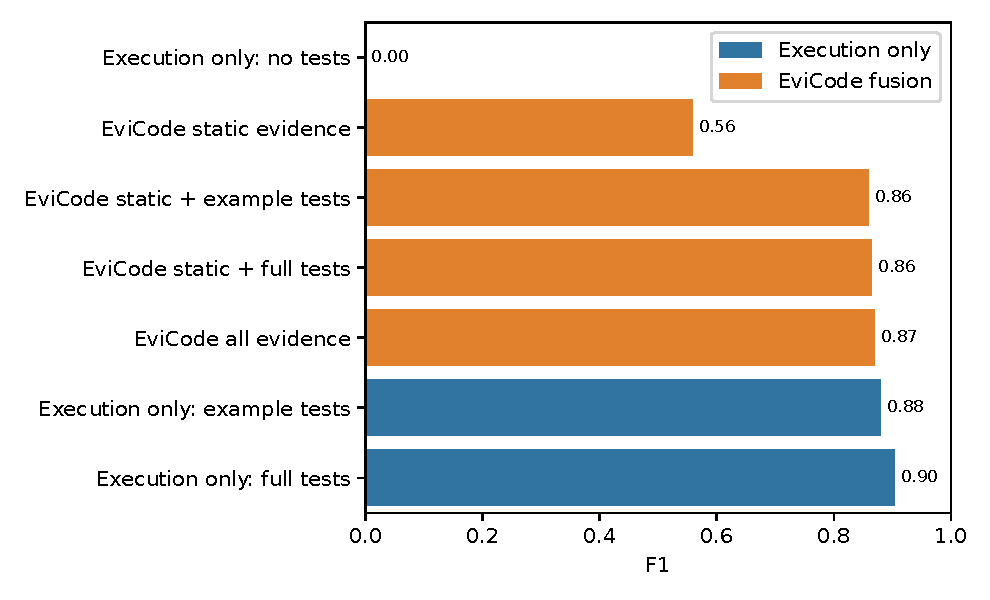
\includegraphics[width=\linewidth]{../figures/execution_budget_curve.pdf}}{\fbox{Execution budget curve not yet generated}}
  \caption{What changes when tests first become available. The large jump from static screening to example execution shows that even limited behavioral observation removes uncertainty unavailable from program form; full tests add a smaller further gain.}
  \label{fig:execution-budget}
\end{figure}

Figure~\ref{fig:execution-budget} therefore uses a discrete evidence-setting comparison rather than a continuous curve. It compares what the dataset can actually support: static-only evidence at F1 0.558, execution-only example tests at 0.879, execution-only full tests at 0.904, and the fused static-plus-execution settings discussed above. The absence of 1, 3, 5, and 10-test rows is intentional: those settings would require separable, normalized assertions that the benchmark does not expose. If future work wants to answer how much execution is necessary, benchmarks need to publish tests as budgetable units rather than only as aggregate harnesses.


\subsubsection{Deployment Depends on Availability, Not Only Accuracy}
The execution-budget results imply a staged deployment model. A system can begin with cheap static screening, run example-level tests when available, and reserve full execution for candidates that remain plausible or high risk. Execution is therefore a resource to allocate according to confidence, cost, and failure risk, rather than a binary capability assumed to be free.

The broader implication of RQ3 is that observation value depends on both information and availability. Execution is strongest but requires the most infrastructure. Cheap static observations are most useful during triage or under constrained test budgets. Their remaining value is diagnostic, which leads to RQ4: can they explain why a candidate deserves scrutiny rather than merely lower its score?

\subsection{RQ4: Can Static Evidence Explain Failures?}
\subsubsection{Representative Evidence Disagreements}
Table~\ref{tab:qualitative-cases-12} expands the qualitative sample to 12 cases, two from each diagnostic group: operator-evidence disagreement, API mismatch, identifier-role mismatch, control-flow mismatch, example/full execution disagreement, and structurally similar but execution-failing programs. Cases are selected deterministically from negative examples satisfying predeclared evidence thresholds. The sample illustrates why the ladder is useful: candidates can preserve AST shape while changing operators or behavior; example tests can agree while full tests disagree; and low role or control similarity localizes a different uncertainty than API mismatch.

\IfFileExists{../tables/qualitative_cases_12.tex}{\begin{table*}[t]
\centering
\footnotesize
\caption{Twelve representative evidence disagreements, two per diagnostic group. Stable case identifiers map to full example IDs in the artifact. Groups are not independently adjudicated causal labels.}
\label{tab:qualitative-cases-12}
\begin{tabular}{llllll}
\toprule
Diagnostic group & Case & Pair & Negative & Ex. & Full \\
\midrule
Operator & C01 & js->java & mismatch & no & no \\
Operator & C02 & java->js & mismatch & no & no \\
API & C03 & java->js & mismatch & no & no \\
API & C04 & java->js & mismatch & no & no \\
Identifier role & C05 & js->python & mismatch & no & no \\
Identifier role & C06 & java->js & mutation & no & no \\
Control flow & C07 & java->python & mismatch & no & no \\
Control flow & C08 & java->js & mutation & yes & yes \\
Ex./full disagree & C09 & java->python & mutation & yes & no \\
Ex./full disagree & C10 & js->python & mutation & yes & no \\
Structural + wrong & C11 & java->js & mutation & no & no \\
Structural + wrong & C12 & java->python & mutation & no & no \\
\bottomrule
\end{tabular}
\end{table*}
}{}

These are representative observations, not independently adjudicated causal bug labels. Several are synthetic mismatches or mutations, and one case can plausibly have multiple causes. We therefore use them to demonstrate auditable evidence disagreement, not to estimate the prevalence or precision of failure categories.

\subsubsection{Explainability Ablation}
Prediction ablation asks whether a family changes accuracy; explainability ablation asks whether removing it erases a diagnostic distinction. Table~\ref{tab:explainability-ablation} removes one family at a time from six rule-defined diagnostic groups. Removing API, control, identifier, operator, or structure evidence eliminates one supported category. Removing execution eliminates two: partial/full execution disagreement and structurally plausible but behaviorally failing candidates. Trigger retention also falls from 3,355 with all families to 1,586 without API evidence and 2,814 without execution. Thus, evidence contributes diagnostic vocabulary even when its marginal F1 effect is small.

\IfFileExists{../tables/explainability_ablation.tex}{\begin{table}
\caption{Diagnostic-retention ablation. Counts refer to rule-defined evidence triggers, not human-adjudicated root-cause accuracy.}
\label{tab:explainability-ablation}
\begin{tabular}{lrrr}
\toprule
Removed & Ret. & Lost & Triggers \\
\midrule
None & 6 & 0 & 3355 \\
Api & 5 & 1 & 1586 \\
Control & 5 & 1 & 2985 \\
Execution & 4 & 2 & 2814 \\
Identifier & 5 & 1 & 2978 \\
Operator & 5 & 1 & 3057 \\
Structure & 5 & 1 & 2842 \\
\bottomrule
\end{tabular}
\end{table}
}{}

The ablation measures retention of rule-defined diagnostic triggers, not how many root causes are ``correctly'' identified; the benchmark has no human root-cause ground truth. Independent annotation is required before making that stronger claim. Within this boundary, the result supports a precise design criterion: an evidence source is useful when removing it makes a relevant class of disagreement unobservable.

The broader implication of RQ4 is that verification should not stop at a correctness label. Decomposed observations turn incorrect outputs into diagnosable cases, which matters when the next action is repair or review. Explanation alone, however, does not establish whether the reported confidence can guide such decisions. The final part of RQ4 therefore tests its probabilistic meaning.

\subsubsection{Confidence Calibration}
Ranking asks which candidate looks more plausible; calibration asks whether confidence such as 0.8 corresponds to roughly 80\% correctness. Figure~\ref{fig:confidence-histogram-calibration} tests that interpretation on held-out data. Of 900 pairs, 536 lie below 0.1 confidence and none is positive, so low-confidence rejection is sharply separated. Sparse bins from 0.2--0.5 are underconfident: actual correctness is 0.80--0.89 despite confidence of only 0.24--0.45. The 0.7--0.9 region is close to calibrated, while the 0.9--1.0 bin is slightly overconfident (0.937 confidence versus 0.909 correctness). A single average error would hide these operating regions.

\begin{figure}[!htbp]
  \centering
  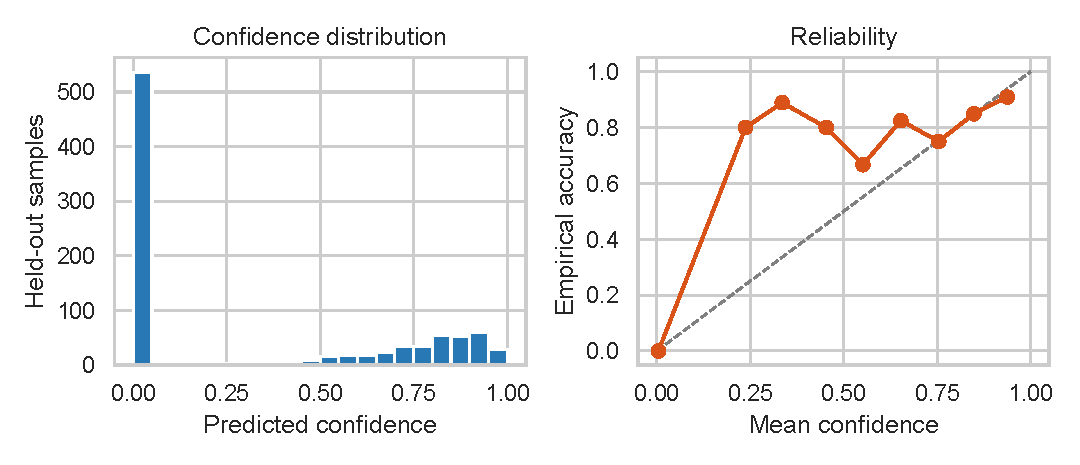
\includegraphics[width=\linewidth]{../figures/confidence_histogram_calibration.pdf}
  \caption{Where confidence is concentrated and whether it matches correctness on held-out data. The large low-confidence mass is reliably incorrect, while sparse middle bins and slight high-end overconfidence identify operating regions that a single average error would hide.}
  \label{fig:confidence-histogram-calibration}
\end{figure}

The calibration result completes RQ4 by separating two forms of interpretability. Decomposed observations explain why confidence moved, while reliability analysis establishes where its magnitude can and cannot be read probabilistically. Together they support triage on held-out data without turning confidence into a claim of proof. The discussion now synthesizes what the four questions collectively reveal about semantic information accumulation.

\section{Supporting Analyses and Discussion}
The four questions examine information, complementarity, cost, explanation, and calibration as parts of one argument. Their common lesson is that a score is meaningful only when the observation behind it matches the decision being made. Static source--candidate observations support ranking, triage, and explanation before execution, while behavioral observations provide the strongest reduction in uncertainty on tested inputs.

Statistical validation prevents overclaiming. Static F1 is 0.558 with a 95\% bootstrap interval of [0.504, 0.612], while execution-heavy configurations are clustered much higher: Example execution 0.879 [0.853, 0.904], All 0.869 [0.840, 0.896], and FullExec 0.904 [0.879, 0.925]. The robust conclusion is the separation between static-only and behavior-observing evidence, not a large thresholded F1 advantage among execution-heavy variants. McNemar tests likewise support a nuanced interpretation: All differs decisively from Static, while small differences among execution-heavy systems should be interpreted cautiously.

\IfFileExists{../tables/bootstrap_f1.tex}{\begin{table}[!htbp]
\centering
\small
\begin{tabular}{lrl}
\toprule
System & F1 & 95\textbackslash \% CI \\
\midrule
All & 0.904 & [0.879, 0.925] \\
FullExec & 0.904 & [0.879, 0.925] \\
Ex. & 0.879 & [0.853, 0.904] \\
Static+Ex. & 0.879 & [0.853, 0.904] \\
Static & 0.454 & [0.394, 0.509] \\
\bottomrule
\end{tabular}
\vspace{0.5em}
\caption{Bootstrap 95\% confidence intervals for selected HumanEval-X F1 scores, estimating uncertainty from resampled held-out predictions.}
\label{tab:bootstrap-f1}
\end{table}
}{}
\IfFileExists{../tables/mcnemar.tex}{\begin{table}[!htbp]
\centering
\small
\begin{tabular}{llrrrr}
\toprule
Baseline & System & B only & S only & Disc. & \$p\$ \\
\midrule
FullExec & All & 0 & 0 & 0 & 1.000 \\
Ex. & All & 18 & 3 & 21 & 0.001 \\
Static & All & 234 & 38 & 272 & 0.000 \\
\bottomrule
\end{tabular}
\vspace{0.5em}
\caption{Exact McNemar tests comparing selected evidence configurations on paired held-out HumanEval-X predictions.}
\label{tab:mcnemar}
\end{table}
}{}

\subsection{Semantic Verification as Information Accumulation}
Across the four questions, the same pattern recurs: verification behaves like inference about an unknown semantic state. Each source supplies a partial observation, and each removes a different uncertainty. Lexical observation identifies shared concepts; syntax removes malformed candidates; structure and control constrain organization and paths; operators, roles, and data flow constrain computation and value movement; execution observes tested outcomes. The experimental findings therefore reveal an \emph{Empirical Semantic Information Ladder}. The ladder was not assumed by the method; it emerged because increasingly direct observations consistently changed what remained unknown.

Figure~\ref{fig:empirical-semantic-ladder} connects this conceptual ordering to measured mean MI, relative mean SHAP importance, incremental held-out F1, and extraction cost. Unlike the broad feature blocks in Table~\ref{tab:evidence-hierarchy}, the figure adds one named observation family at a time; its increments therefore answer a finer-grained question and are not numerically interchangeable with the table's deltas. Execution has mean MI 0.420 and adds 0.314 F1 after the accumulated static levels. Earlier levels make smaller, complementary contributions at much lower cost. Adjacent measurements are not required to be monotonic: correlated evidence can have low marginal MI or even slightly negative incremental F1, as control flow does after preceding levels ($-0.003$), while still removing a distinct uncertainty. The empirical principle is progressive observability, not a claim that every additional feature must improve every finite-sample metric.

\begin{figure*}[!t]
  \centering
  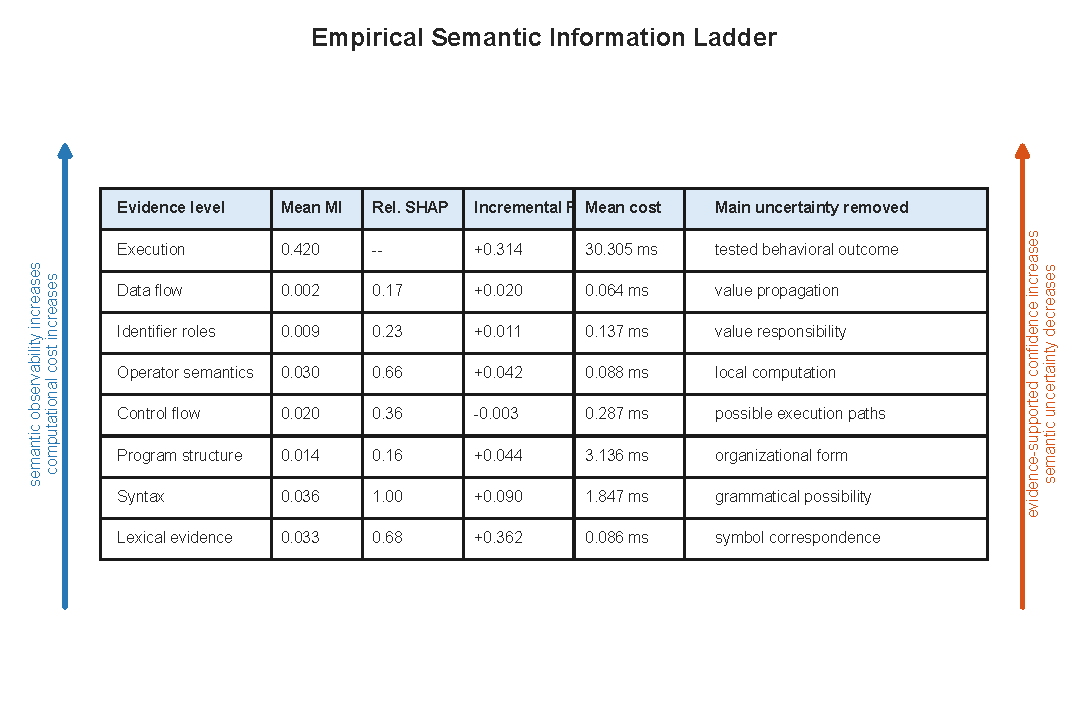
\includegraphics[width=0.96\textwidth]{../figures/empirical_semantic_information_ladder.pdf}
  \caption{\textbf{Empirical Semantic Information Ladder.} Moving upward generally increases semantic observability, acquisition cost, and evidence-supported confidence while reducing uncertainty. Each row retains measured information, static-model use, incremental F1, cost, and the uncertainty addressed. Individual timings and predictive increments need not be monotonic because extractors differ in implementation and observations can be redundant; execution SHAP is omitted because SHAP intentionally analyzes the static model.}
  \label{fig:empirical-semantic-ladder}
\end{figure*}

This information-accumulation view separates verification from similarity scoring. Similarity is one possible observation near the bottom of the ladder; verification combines partial observations until uncertainty is low enough for prioritization, review, or tested acceptance. Static evidence should survive when it exposes a distinct uncertainty, and confidence should be audited under the conditions where it will be used.

The ladder describes information content, but a deployed verifier must also decide \emph{when} to acquire each observation. Figure~\ref{fig:evidence-acquisition-timeline} turns the discovery into a staged decision process. Cheap observations arrive first and support filtering; richer static observations refine diagnosis; execution is delayed until its higher cost is justified; the final decision is made from both what has been observed and what remains uncertain.

\begin{figure*}[!t]
  \centering
  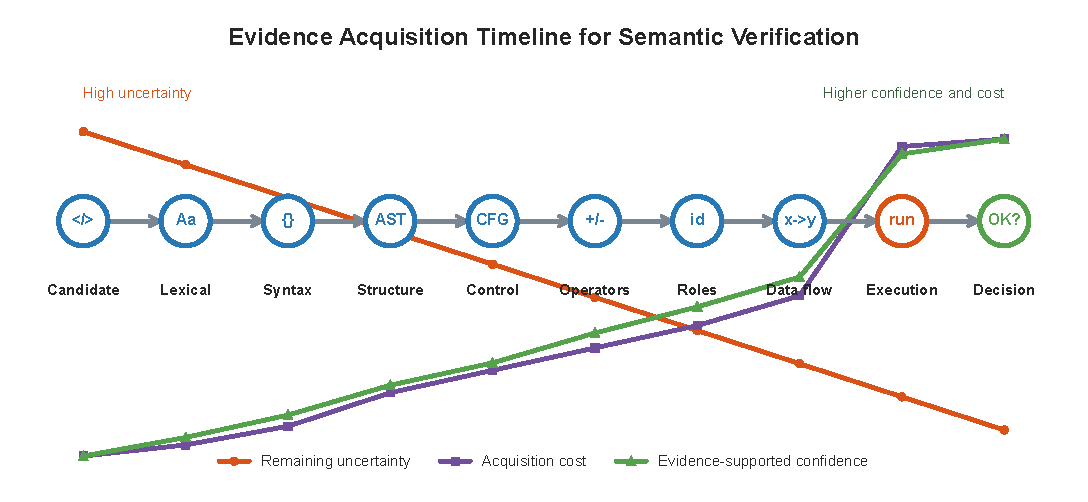
\includegraphics[width=0.96\textwidth]{../figures/evidence_acquisition_timeline.pdf}
  \caption{\textbf{Evidence Acquisition Timeline for Semantic Verification.} A candidate is examined through increasingly informative observations before a decision is made. The curves are qualitative, not additional measurements: remaining uncertainty falls, while acquisition cost and evidence-supported confidence generally rise. The timeline summarizes the practical lesson of the empirical ladder---acquire cheap observations early and pay for execution when unresolved risk justifies it.}
  \label{fig:evidence-acquisition-timeline}
\end{figure*}

\subsection{What EviCode Does Not Claim}
EviCode does not prove semantic equivalence, replace formal verification, replace execution, or claim that static evidence alone is sufficient. Test outcomes remain bounded by their inputs, and static features remain approximations. EviCode instead quantifies available semantic evidence, measures uncertainty reduction, explains which observations influence a decision, supports candidate prioritization, and guides where execution resources may be spent. These uses are deliberately narrower than certification and broader than reporting one similarity score.

\section{Threats to Validity}
\textbf{Construct validity.} HumanEval-X correctness approximates semantic correctness through tests. Passing tests is not full equivalence, and failing tests may reflect harness issues. Static evidence features are approximations rather than formal analyses. HumanEval-X exposes example and full test programs, but not a normalized list of individual assertions across all target languages; the paper therefore reports completed execution-availability settings rather than fabricating retained-test curves.

\textbf{Internal validity.} Negative HumanEval-X examples are created by mismatch and mutation, which may make some failures easier than real model errors. Grouped problem-level splits reduce leakage across tasks, but feature extraction bugs or parser limitations could affect results.

\textbf{Explanation validity.} The failure categories are derived from observable evidence rules rather than from independent human root-cause annotation. They are useful for diagnosing where a verifier's evidence disagrees, but they should not be interpreted as complete semantic bug explanations. Manual annotation of a stratified sample of negative and disagreement cases would further validate the precision of these explanations.

\textbf{External validity.} The benchmark covers short Python, Java, and JavaScript HumanEval-X tasks. Results may differ for larger systems, interactive programs, domain-specific APIs, other language paradigms, or naturally occurring model errors. Evaluating whether evidence relationships and calibration remain stable under model and dataset shift is future work rather than a claim of this study.

\textbf{Conclusion validity.} The study uses bootstrap intervals and McNemar tests, but some comparisons remain exploratory. Coefficients and SHAP values explain model use, not causal semantic importance. Static cost measurements use Python allocation tracing; execution timing excludes unavailable Java runs and does not capture child-process memory.

\textbf{Ecological validity.} Real development workflows involve human review, build systems, dependencies, and evolving requirements. EviCode models the verification core, not the full socio-technical workflow.

\section{Conclusion}
The central lesson is that semantic verification can be understood as progressive accumulation of heterogeneous evidence, with each source removing a different component of uncertainty. Lexical form and syntax provide weak but inexpensive screening; structure, control, operators, roles, and data flow reveal increasingly specific program obligations; and execution observes tested consequences. Static evidence does not prove equivalence. Its value is early uncertainty reduction, prioritization, and explanation when no reference translation or test suite exists.

Future verification systems should therefore be organized around the information each observation contributes, the uncertainty it leaves behind, the cost required to acquire it, and the other evidence needed to interpret it. A universal intermediate representation could make normalization less dependent on parser-specific approximations; static single assignment (SSA) and program-dependence graphs could strengthen value-flow observations; symbolic execution and formal semantics could add observations between static proxies and concrete execution; and graph neural models could test whether richer fusion recovers the same hierarchy without sacrificing auditability. The same evidence-accumulation questions should also be studied for larger programs, C-to-Rust migration, Defects4J repair, and other generation settings. These are tests of the ladder's scope, not assumptions that its ordering is universal.

Verification should therefore not begin and end with the binary question ``is this code correct?'' It should ask what has been observed, what semantic uncertainty remains, and whether acquiring the next observation is worth its cost.

\bibliographystyle{IEEEtran}
\bibliography{references}

\appendices
\section{Reproducibility Checklist}
The repository includes dependency manifests, setup documentation, resume-safe progress files, unit tests, benchmark outputs, fixed split assignments, grouped-bootstrap outputs, generated tables and figures, and a reproducible paper build path. Exploratory artifacts remain available in the repository but are not part of the main-paper evaluation.

\end{document}

